\makeatletter
\newcommand\HUGE{\@setfontsize\Huge{20}{30}}
\makeatother    
 
\newcommand{\Titolo}{Computational Mathematics for Learning and Data Analysis}

\newcommand{\Gruppo}{Federico Finocchio\\\texttt{f.finocchio@studenti.unipi.it}}
\newcommand{\norm}[1]{\left\lVert #1 \right\rVert_2}

\documentclass[a4paper, oneside, openany]{article}
\usepackage[backend=biber, sorting=none]{biblatex}
\addbibresource{bibliography.bib}
\usepackage{setspace}
\usepackage{todonotes}
\usepackage{titling}
\usepackage{graphbox}
\usepackage{amsmath , amssymb , amsthm}
\usepackage{comment} 
% permette di modificare i margini
\usepackage[top=2cm, bottom=2cm, left=2.cm, right=2.cm]{geometry}
\newgeometry{top=3.4cm}


\newtheoremstyle{myplain}
  {\topsep}   % ABOVESPACE
  {\topsep}   % BELOWSPACE
  {\itshape\onehalfspacing}  % BODYFONT
  {0pt}       % INDENT (empty value is the same as 0pt)
  {\bfseries} % HEADFONT
  {.}         % HEADPUNCT
  {5pt plus 1pt minus 1pt} % HEADSPACE
  {}       
\theoremstyle{myplain}
\newtheorem{thm}{Theorem}[section]
\theoremstyle{plain}
\newtheorem{assumption}{Assumption}[subsection]
\newtheorem{lemma}[thm]{Lemma}

\usepackage{lastpage} %info sul # dell'ultima pagina del documento
\usepackage{fancyhdr} %per modificare dimensioni,margini, intestazioni e righe a piè di pagina
\fancypagestyle{plain}{
  % cancella tutti i campi di intestazione e piè di pagina
  \fancyhf{}
  
  \cfoot{Page \thepage{} of \pageref{LastPage}} %es: pag: 4 di 10

  %linea orizzontale alle posizioni top e bottom della pagina
  \renewcommand{\headrulewidth}{0 pt}  
  \renewcommand{\footrulewidth}{0 pt}
}
\pagestyle{plain} 

%\usepackage{calc} %introduce la notazione infissa per le op. aritmetiche interne a LaTeX

\usepackage[utf8]{inputenc}
\usepackage[T1]{fontenc}
\usepackage[english]{babel} %il documento è in italiano

\usepackage{graphicx}       %permette di inserire delle immagini
\usepackage{caption}        %numerazione figure e loro descrizione testuale
\usepackage{subcaption}     %sottofigure numerabili
\usepackage{float}  %permette di inserire un # qualsiasi di figure fluttuanti
\usepackage{xcolor}
\usepackage{rotating} %permette di ruotare le immagini

%package utili per la math mode ( $ ... $ o \[ ...  )
\usepackage{amsmath}
\usepackage{amssymb}
\usepackage{amsfonts}
\usepackage{amsthm}
\usepackage{mathtools}

% package utili per tabelle(\thead in particolare)
\usepackage{array, booktabs, caption}
\usepackage{makecell}
\renewcommand\theadfont{\bfseries}
\usepackage{boldline}

\usepackage{listings} %permette di inserire degli spezzoni di codice

\usepackage{tikz} %disegno di immagini vettoriali a schermo. Utile per grafi
\usetikzlibrary{arrows.meta}
\usetikzlibrary{graphs}
\usetikzlibrary{arrows}
%\usepackage{tikz-uml} %serve per disgnare l'UML, fantastica guida:
%https://perso.ensta-paristech.fr/~kielbasi/tikzuml/var/files/doc/tikzumlmanual.pdf
%download package: http://perso.ensta-paristech.fr/~kielbasi/tikzuml/
\usepackage{fix-cm}    
%package per le tabelle
\usepackage{booktabs} %permette di poter usare delle liste nelle tabelle
\usepackage{tabularx} 
\usepackage{longtable} %una tabella può continuare su più pagine
\usepackage{multirow} %utile per visualizzare una cella su più righe
%\usepackage{multicolumn} %cella su più colonne
%\usepackage[table]{xcolor} %rende disponibile l'utilizzo di un colore per lo sfondo
                        %delle celle di una tabella

%crea una cella per le tabelle in grado di andare a capo con \newline
%https://tex.stackexchange.com/questions/12703/how-to-create-fixed-width-table-columns-with-text-raggedright-centered-raggedlef
\usepackage{array}
\newcolumntype{L}[1]{>{\raggedright\let\newline\\\arraybackslash\hspace{0pt}}m{#1}}
\newcolumntype{C}[1]{>{\centering\let\newline\\\arraybackslash\hspace{0pt}}m{#1}}
\newcolumntype{R}[1]{>{\raggedleft\let\newline\\\arraybackslash\hspace{0pt}}m{#1}}


%indice con i puntini
\usepackage{tocloft}
\renewcommand\cftsecleader{\cftdotfill{\cftdotsep}}

%http://ctan.mirror.garr.it/mirrors/CTAN/macros/latex/contrib/appendix/appendix.pdf
\usepackage{appendix} %aggiunge dei comandi per l'appendice
\usepackage{parskip} %aiuta LaTeX a trovare il miglior stile per i page break
\setcounter{secnumdepth}{5} % numera i sottoparagrafi
\setcounter{tocdepth}{5} %aggiunge all'indice i sottoparagrafi
%\usepackage{titlesec} %\begin{paragraph} si può usare come subsubsubsection!


\usepackage{breakurl}%\url{...} può continare alla linea successiva. (si può andare a capo)

\definecolor{Maroon}{cmyk}{0, 0.87, 0.68, 0.32}
\usepackage[colorlinks=true]{hyperref}
\hypersetup{
    colorlinks=true,
    citecolor=black,
    filecolor=black,
    linkcolor=black, % colore dei link interni
    urlcolor=Maroon  % colore dei link interniesterni
}

%impostazioni per il codice che deve finire dentro a
%\begin{lstlisting}

\definecolor{listinggray}{gray}{0.9}
\definecolor{lbcolor}{rgb}{0.9,0.9,0.9}
\lstset{
backgroundcolor=\color{lbcolor},
    tabsize=4,    
%   rulecolor=,
    language=[GNU]C++,
    basicstyle=\scriptsize,
    upquote=true,
    aboveskip={1.5\baselineskip},
    columns=fixed,
    showstringspaces=false,
    extendedchars=true,
    inputencoding=utf8,
    breaklines=true,
    prebreak = \raisebox{0ex}[0ex][0ex]{\ensuremath{\hookleftarrow}},
    frame=single,
    numbers=left,
    showtabs=false,
    showspaces=false,
    showstringspaces=false,
    identifierstyle=\ttfamily,
    keywordstyle=\color[rgb]{0,0,1},
    commentstyle=\color[rgb]{0.026,0.112,0.095},
    stringstyle=\color[rgb]{0.627,0.126,0.941},
    numberstyle=\color[rgb]{0.205, 0.142, 0.73},
%        \lstdefinestyle{C++}{language=C++,style=numbers}’.
}
\lstset{
  backgroundcolor=\color{lbcolor},
  tabsize=4,
  language=C++,
  captionpos=b,
  tabsize=3,
  frame=lines,
  numbers=left,
  numberstyle=\tiny,
  numbersep=5pt,
  breaklines=true,
  showstringspaces=false,
  basicstyle=\footnotesize,
  identifierstyle=\color{magenta},
  keywordstyle=\color[rgb]{0,0,1},
  commentstyle=\color{orange},
  stringstyle=\color{red}
}

\usepackage{algorithm}% http://ctan.org/pkg/algorithms
\usepackage{algpseudocode}% http://ctan.org/pkg/algorithmicx


\begin{document}

\begin{titlepage}
	\begin{center}
		
		\vspace{1cm}
	
		\begin{HUGE}
		
			\Titolo{} \\
		\end{HUGE}
		
		\vspace{13pt}  
		
		\begin{large}
		\Gruppo{}\ \\	
		\end{large}
		
		\vspace{10pt}
		    
		\begin{large}
			A.Y. 2020/2021
		\end{large}  
		
	\end{center}
	\vspace{1cm}
\begin{abstract}
\textit{Assigned project: ML project 6}\newline
(M1) is a neural network with topology of your choice, but mandatory piecewise-linear activation function (of your choice); any regularization is allowed.\newline
(M2) is a standard L\_2 linear regression (min least squares).\newline
(A1) is a standard momentum descent approach applied to (M1).\newline
(A2) is an algorithm of the class of deflected subgradient methods applied to (M1).\newline
(A3) is a basic version of the direct linear least squares solver of your choice (normal equations, QR, or SVD) applied to (M2).
\end{abstract}
\end{titlepage}

\restoregeometry

\section{Introduction}
This report is about the project assigned for the course of Computational Mathematics for Learning and Data Analysis. All the work in this project is the result of the knowledge gathered from the courses of \textbf{ML} and \textbf{CM}. The report contents that are not directly work of the authors is referenced and, as requested, we point to the references down to chapter and number of page (when necessary).

We start by giving a short description of the problem at hand and the methods used to solve it, including all the mathematical derivation needed to adapt the chosen methods to the problem. Next, we give a brief recap of the expected results for the experiments, properties of the problem that suits our methods and details about the solvability of our problem with the used methods. In the end, we show the achieved results, comparing them with the expected one describing which are the factors that determined a difference in the results.

The models to be implemented are:
\begin{itemize}
    \item \textbf{M1}: a neural network, \textit{ANN} in the following, with piecewise-linear activation function, with possible regularization;
    \item \textbf{M2}: standard L\_2 linear regression
\end{itemize}
The methods to be applied to the models are:
\begin{itemize}
    \item \textbf{A1}: standard momentum descent approach applied to \textbf{M1};
    \item \textbf{A2}: deflected subgradient methods applied to \textbf{M1};
    \item \textbf{A3}: basic version of one of the direct linear least squares solvers (i.e. normal equations, QR, SVD) applied to \textbf{M2}.
\end{itemize}
In the following we describe the main implementation choices and introduce some of the notation used in the rest of the report. The detailed description of the implemented methods is given in the related sections of this document.
\section{Project structure and notation}
The main aim of this project was to build two application models and apply different optimization methods to the implemented models.\newline
The models to be implemented are:
\begin{itemize}
    \item \textbf{M1}: a neural network with piecewise-linear activation function, with possible regularization;
    \item \textbf{M2}: standard L\_2 linear regression
\end{itemize}
The methods to be applied to the models are:
\begin{itemize}
    \item \textbf{A1}: standard momentum descent approach applied to \textbf{M1};
    \item \textbf{A2}: deflected subgradient methods applied to \textbf{M1};
    \item \textbf{A3}: basic version of one of the direct linear least squares solvers (i.e. normal equations, QR, SVD) applied to \textbf{M2}.
\end{itemize}
In the following we will describe what are the main implementation choices and introduce some of the notation used in the rest of the report.\newline
As requested, the project requires to implement from scratch an \textit{Artificial Neural Network}, \textit{ANN} in the following and as referred in \cite{MLmitchell}, and a direct solver for the linear least square problem. The detailed description of the implemented methods will be given in the related sections of this document.
\section{Artificial Neural Network}
The notation used to refer The implemented \textit{ANN} can be seen as a \textit{fully connected multilayer Perceptron} as referred in the literature and as shown in \cite{MLmitchell}. An \textit{ANN} is composed by an interconnection of units that can represented as the composition of two functions that will determine the real-valued output of \todo{magari descrivere che cosa è un perceptron}the unit. The two functions will be referred as the \textit{network function} and the \textit{activation function}, where the former computes the scalar product of the input vector with the weight vector of the current unit, the latter is the function that will directly determine the output of the current unit. As we will see, the choice of the activation function is particularly important and is preferred to be a nonlinear combination of its inputs, maintaining the property of being differentiable.

The implemented \textit{ANN} will be structured with multiple layers, each layer will have all the units fully connected with the adjacent layers and, as convention, we will refer to the first layer as \textit{input layer} and to the last layer as \textit{output layer}. The others will be referred as \textit{hidden layers}. Another important aspect when implementing an \textit{ANN} is the choice of the number of units. Later in this report will be shown how the exact number of units in each layer will be chosen, but we can already describe the structure of the input and the output layer. The former will contain a number of units that is the same as the number of features contained in the data that will be fed up to the \textit{ANN}, instead the latter will contain one binary output units for classification tasks and one real-output unit for regression tasks.\newline

In the following sections we will describe in more details which are the main aspects of the implemented \textit{ANN} like the network structure, the functions used to compute the output of each unit and the algorithm used to let the network learn the task at hand.

\subsection{Network structure}
As already pointed out in the previous section, the network structure will be composed of multiple layers. The number of layers and consequently, the number of units per layer will be determined by an empirical approach that will target the minimization of the empirical error on the tested data. This will be explained in more detail in the testing section.\newline

The input and the output layer will be of fixed dimensions, as the number of units for the former will be determined by the size of the input data and the dimension of the latter will be determined by the task to be completed. As we will see, the number of units in the output layer will be always of one, what will change instead is the type of the units, because for classification tasks we will use a binary unit, instead for a regression task we will use a real-output unit.

\subsection{Activation function}
The choice of the activation function is a crucial step for the construction of the \textit{ANN}. This function will directly determine what is the output of each of the units in the network, depending on the result of the scalar product of the unit input and the unit weights vectors. The activation function, to be useful, needs to have determined properties, like differentiability, \textbf{AGGIUNGERE ALTRE PROPRIETà CHE LA RETE DEVE AVERE}.\newline

The mainly used ones, which will be used also for the purposes of this project, are:
\begin{itemize}
    \item Sigmoid
    \item TanH
\end{itemize}

\subsection{Loss function}
The loss function is used to estimate the error at the output of the network given the vector of the expected values for the data that are fed up into the network. The loss function is also the function to be minimized as the main aim for the learning algorithm. The error computed via the loss function is usually used as a termination condition for the learning algorithm. This is done via various algorithm, and in particular for our case via subgradient methods and standard momentum descent approach.\newline

In our case we decided to use as a function to measure the error in the prediction the \textit{MSE} that represents the sum, over all the available data, of the squared differences between the predicted value and the actual one.\newline

\subsubsection{Derivation of Loss function}
As a preliminary step for the backpropagation algorithm, we illustrate here how the gradient of the loss function is computed. The result is then used to update the value of the weight vector for each unit. In the following the derivation of the loss function.\newline\newline
\textbf{QUI INSERIRE DERIVAZIONE LOSS FUNCTION}

\subsection{Backpropagation algorithm}
The backpropagation algorithm \cite{haykin_neural_2009} is used to learn weight vectors for a multilayer network, given the network inputs and the fixed network structure (i.e. units and interconnections). This algorithm employs a gradient descent approach to attempt to minimize the squared error between the network output values $\textbf{y}$ and the target values $\hat{\textbf{y}}$ associated to these outputs. This algorithm is described in \cite{MLmitchell} and is composed by two main parts:
\begin{itemize}
    \item \textbf{Forward phase}: data traverse the network from the input units to the output units, in such a way the result of the network with the given input and the current weight vector value can be compared to the expected output to estimate the error;
    \item \textbf{backward phase}: the gradient of the loss function is used to update the weight vectors of each layer in a way that the next step will have a smaller value for the error function.
\end{itemize}
The main aim for the backpropagation algorithm is to minimize the error function via automatic fine-tuning of the weight vector. This minimization can be achieved in different ways utilizing the gradient of the loss function computed with the results obtained with the forward phase.\newline
\cite{MLmitchell}

\section{Least Square}
\label{sec:ls}
The \textit{Least Square problem} is described in \parencite[Lecture 11]{Bau} and \parencite[Chap. 3]{elden} as the problem of finding a solution of an overdetermined system of equations $Ax = b$ by finding a vector $x$ that minimizes the 2-norm of the residual vector defined as $r = b - Ax$.

The \textit{Least Square problem}, given $A\in\mathbb{R}^{m\times n},\ m\geq n,\ b\in\mathbb{R}^m$, has the following form:
\begin{equation}
    \label{eq:ls}
    \text{find}\ x\in\mathbb{R}^n\ \text{that solves the minimization problem}\ \min_{x}\norm{b - Ax}\ \text{.}
\end{equation}
We describe in section \S\ref{sec:qr}, related to the implemented direct solver, that this kind of problems have a unique solution if the matrix $A$ has \textit{full column rank}.
\section{Methods}
This section gives detailed information about the required methods that will be implemented and applied to the models described in \S\ref{sec:ann} and \S\ref{sec:ls}. The main methods to be implemented are:
\begin{itemize}
    \item Standard momentum descent approach applied to the \textit{ANN};
    \item Deflected subgradient method applied to the \textit{ANN};
    \item Direct linear least square solver applied to the \textit{Least Square problem}.
\end{itemize}

\subsection{Momentum method}
The momentum approach is a technique that accelerates the gradient descent accumulating a velocity vector in directions of persistent reduction \cite{momentum}.

We can define \textit{Classical Momentum} (CM) as:
\begin{align}
    & v_{t+1} = \mu v_t - \epsilon \nabla f(\Theta_t) \\
    & \Theta_{t+1} = \Theta_t + v_{t+1}
\end{align}
where $\epsilon > 0$ is the learning rate, $\mu \in [0,1)$ is the momentum coefficient and $\nabla f(\Theta_t)$ is the gradient at $\Theta_t$. The hyperparameter of momentum determines how quickly the contributions of previous gradients exponentially decay.  Another important aspect is that the larger $\mu$ is, relative to $\epsilon$, the more previous gradients affect the current direction. At the moment, no prior choices of the momentum coefficient and learning rate can be done, these will be studied more in the detail in a later phase of the project where we implement and test these models, but as suggested by \parencite[Chap. 8]{bengio}, common values for $\mu$ are $0.5, 0.9, 0.99$.

The next algorithm is the pseudocode relative to the \textit{Gradient descent with momentum}, given the learning rate and the momentum coefficient, performs a descent approach until termination conditions are met.
\begin{algorithm}[H]
	\caption{Gradient descent with momentum. Termination conditions, learning rate and momentum coefficients have to be determined by testing as it will be shown in a later phase of the project. For the moment we assume that they are given.}
	\label{alg:gdmom}
	\begin{algorithmic}[1]
		\State Initialize $\mathit{\Theta}$ and $\mathbf{v}$
		\While{$termination\ conditions\ not\ met$}
		\State Sample $m$ examples $(x_1,y_1), (x_2,y_2) \dots (x_m,y_m)$
		\State $\mathit{\Tilde{\Theta}} \leftarrow \mathit{\Theta}$
		\If {$Nesterov$}
		\State $\mathit{\Tilde{\Theta}} \leftarrow \mathit{\Tilde{\Theta}} + \mu \mathbf{v}$
		\EndIf
		\State Compute gradient estimate: $\mathbf{g} \leftarrow \frac{1}{m}\nabla_{\mathit{\Tilde{\Theta}}}\sum_i(L(f(x_i,\mathit{\Tilde{\Theta}}),y_i))$
		\State Compute velocity update: $\mathbf{v} \leftarrow \mu \mathbf{v} - \epsilon g$
		\State Apply update: $\mathit{\Theta} \leftarrow \mathit{\Theta} + \mathbf{v}$
		\EndWhile
	\end{algorithmic}
\end{algorithm}
In \hyperref[alg:gdmom]{Algorithm \ref{alg:gdmom}} the amount of samples taken at \textit{line 3} determines the type of \textit{Gradient descent algorithm}, such as:
\begin{itemize}
    \item $\mathbf{m = 1}$: \textit{stochastic gradient descent (SGD)};
    \item $\mathbf{m < n}$, where n is the total number of examples: \textit{batch stochastic gradient descent};
    \item $\mathbf{m = n}$: \textit{standard gradient descent (GD)}.
\end{itemize}
A further improvement is given by a modification of the \textit{CM} approach, called \textit{Nesterov's Accelerated Gradient} (NAG) that, seen as a momentum approach, can be defined as:
\begin{align}
    \label{eq:nag}
    & v_{t+1} = \mu v_t - \epsilon\nabla f(\mathit{\Theta_t} + \mu v_t) \\ 
    & \mathit{\Theta_{t+1} = \mathit{\Theta_t} + v_{t+1}}
\end{align}
The only difference from \textit{CM }is relative to the point where the gradient is computed, in fact NAG performs a partial update to $\mathit{\Theta_t}$ and uses this update to compute the gradient at step $\mathit{t}$. After computing the gradient, the update rule is the same, but in this way NAG allow changing $v$ in a more responsive way. This modification is implemented in \hyperref[alg:gdmom]{Algorithm \ref{alg:gdmom}} at \textit{line 6} where an update to the point of evaluation of the gradient is performed. Differences between \textit{CM} and \textit{NAG} can be seen in \hyperref[fig:NAGvsCM]{\textbf{Figure \ref{fig:NAGvsCM}}}.
\begin{figure}[H]
	\centering
	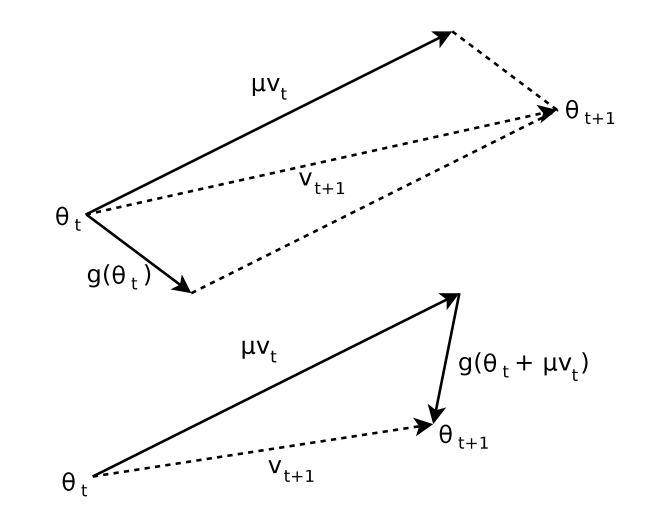
\includegraphics[width=0.4\linewidth]{res/CMvsNAG.png}
	\caption{\textit{\textit{CM} (on top) shows how the update of the vector $v_t$ using the gradient at $\Theta_t$ differs from the \textit{NAG} (on bottom). When $\mu v_t$ is a poor update, we can see how \textit{NAG} points $v_{t+1}$ back towards $\Theta_t$ more strongly than \textit{CM}.}}
	\label{fig:NAGvsCM}
\end{figure}

\subsubsection{Convergence}
\label{conv_mom}
As shown in \cite{momentum}, \textit{NAG} can help avoiding oscillations in the path taken by \textit{CM}. In \hyperref[fig:convNAGvsCM]{\textbf{Figure \ref{fig:convNAGvsCM}}} we can see the comparison between the two momentum methods with same momentum and learning rate coefficients. This shows how the correction rule for a poor update, as shown in \hyperref[eq:nag]{Equation \ref{eq:nag}}, over multiple iterations, can help \textit{NAG} to be more effective than \textit{CM} at decelerating over time. This also helps \textit{NAG} to be more tolerant to larger values of $\mu$ compared to \textit{CM}.
\begin{figure}[H]
	\centering
	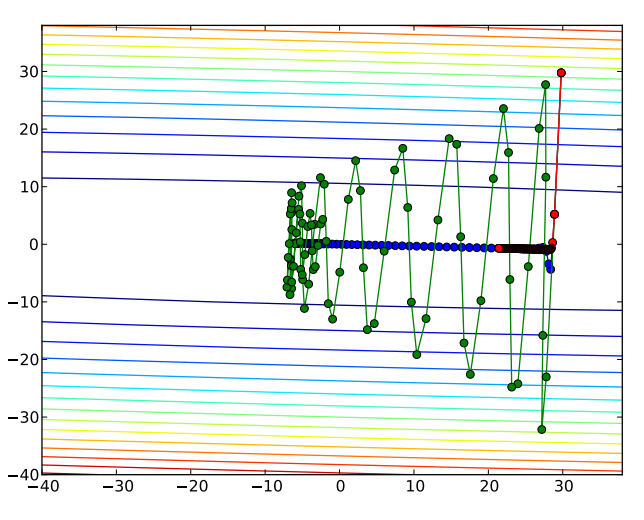
\includegraphics[width=0.4\linewidth]{res/convNAGvsCM.png}
	\caption{\textit{Given the global minimizer of the objective function in (0,0), the red, blue and green curves show, respectively, the trajectories of \textit{gradient descent}, \textit{NAG} and \textit{CM}. It's clearly visible the difference in oscillations between \textit{CM} and \textit{NAG} approach.}}
	\label{fig:convNAGvsCM}
\end{figure}
% To study convergence we can refer to the more generic theorem described in \parencite[Theorem 3.2]{nocedal}:
% \todo[inline]{controllare questo teorema, in teoria non serve a niente come detto da Frangioni in mail}
% \begin{thm}
% \label{thm:zou}
% Consider any iteration of the form $x_{k+1} = x_k + \alpha_k p_k$, where $p_k$ is a descent direction and $\alpha_k$ satisfies the Wolfe conditions. Suppose that f is bounded below in $\mathbb{R}^n$ and that f is continuously differentiable in an open set $\mathit{N}$ containing the level set $\mathit{L} \stackrel{def}{=} \{x:f(x)\leq f(x_0)\}$, where $x_0$ is the starting point of the iteration. Assume also that the gradient $\nabla f$ is Lipschitz continuous on $\mathit{N}$, then
% \begin{align*}
%     & \sum_{k\geq 0}cos^2\Theta_k\norm{\nabla f_k}^2 < \infty
% \end{align*}
% \end{thm}
% Given that for $p_k$ to be a proper descent direction we must have $cos(\Theta_k) > 0$ not too small, we necessarily have that $\norm{\nabla f_k} \rightarrow 0$.

% As shown in \cite{bottou2018opt}, we can guarantee convergence for the \textit{SGD} algorithm applied to a non-convex objective function, which is our case, under certain assumptions. The following assumptions must hold to ensure convergence.
% \begin{assumption}
% \label{ass:conv1}
% The objective function $F:\mathbb{R}^d\to\mathbb{R}$ is continuously differentiable and $\nabla F: \mathbb{R}^d\to\mathbb{R}$ is Lipschitz continuous with Lipschitz constant $L>0$, i.e.
% \begin{align*}
%     \norm{\nabla F(w) - \nabla F(\Bar{w)}} \leq L\norm{w-\Bar{w}}\, \, for\, \, all\, \{w\,,\Bar{w}\} \subset\mathbb{R}^d
% \end{align*}
% \end{assumption}

% \begin{assumption}
% \label{ass:conv2}
% The objective function and SGD satisfy the following:
% \begin{itemize}
%     \item The sequence of iterates $\{w_k\}$ is contained in an open set over which $F$ is bounded below by a scalar $F_{inf}$.
%     \item There exist scalars $\mu_G > \mu > 0$ such that, for all $k\in \mathbb{N}$,
%     \begin{align*}
%         \nabla F(w_k)^T\mathbb{E}_{\xi_k}[g(w_k,\xi_k)] &\geq \mu\norm{\nabla F(w_k)}^2\\
%         \norm{\mathbb{E}_{\xi_k}[g(w_k,\xi_k)]} &\leq \mu_G\norm{\nabla F(w_k)}
%     \end{align*}
%     \item There exist scalar $M \geq 0$ and $M_V \geq 0$ such that for all $k\in\mathbb{N}$,
%     \begin{align*}
%         \mathbb{V}_{\xi_k}[g(w_k,\xi_k)] \leq M + M_V\norm{\nabla F(w_k)}^2
%     \end{align*}
% \end{itemize}
% \end{assumption}

% Under the assumptions \textit{\ref{ass:conv1}} and \textit{\ref{ass:conv2}}, we can use \parencite[Theorem 4.9]{bottou2018opt} to prove convergence of the \textit{SGD} algorithm when used over a non-convex objective function.

% \begin{thm}
% \label{thm:sgdconv}
% Suppose that SGD algorithm is run with a stepsize satisfying ${\sum_{k=1}^\infty\epsilon_k=\infty}$ and $\sum_{k=1}^\infty\epsilon_k^2<\infty$. Then,
% \begin{align*}
%     \liminf\limits_{k\to\infty}\mathbb{E}[\norm{\nabla F(w_k)}^2] = 0
% \end{align*}
% \end{thm}
% From this follows that for the \textit{SGD} method, with diminishing step sizes, the expected value of the gradient norm has to decrease and go to zero.
As stated in \parencite[Chap. 8]{bengio}, under a practical point of view, a sufficient condition to guarantee \textit{SGD} to converge is:
\begin{align*}
    & \sum_{k=1}^\infty\epsilon_k=\infty,\ \sum_{k=1}^\infty\epsilon_k^2<\infty\ \textit{ with $\epsilon_k$ learning rate at step k.}
\end{align*}

To study convergence of the \textit{SGD} involving \textit{CM} and \textit{NAG}, applied to a non-convex objective function, we refer to the results obtained in \cite{sgdunified} that describes a unified framework for both momentum methods. The unified framework uses the constant $s=0$ and $s=1$ to refer, respectively, to \textit{CM} and \textit{NAG}. We define $C>0$ a positive constant and $\mathit{G}_k = \mathit{G}(x_k; \xi_k)$ a stochastic gradient  of $f(x)$ at $x_k$, depending on a random variable $\xi_k$, such that ${\mathbb{E}[\mathit{G}(x_k;\xi_k)] = \nabla f(x_k)}$. The following theorem shows the convergence of \textit{SGD} with momentum for a non-convex objective function $f(x)$.

\begin{thm}[\textit{Convergence of SGD with momentum}]
\label{thm:convmom}
Suppose $f(x)$ is a non-convex and L-smooth function, ${\mathbb{E}[\norm{\mathit{G}(x;\xi)-\nabla f(x)}^2]\leq\delta^2}$ and $\norm{\nabla f(x)}\leq\mathit{B}$ for any $x$. Let the method run for $t$ iterations. By setting $\epsilon = \min\{\frac{1-\mu}{2L[1+((1-\mu)s-1)^2]}\,,\frac{C}{\sqrt{t+1}}\}$ we have:
\begin{align*}
    \min_{k=0,...,t}\mathbb{E}[\norm{\nabla f(x_k)}^2] &\leq \frac{2(f(x_0)-f^*)(1-\mu)}{t+1}\max\Big\{\frac{2L[1+((1-\mu)s-1)^2]}{1-\mu}\,,\frac{\sqrt{t+1}}{C}\Big\}\\
    &+\frac{C}{\sqrt{t+1}}\frac{L\mu^2(\mathit{B}^2+\delta^2)+L\delta^2(1-\mu)^2}{(1-\mu)^3}
\end{align*}
\end{thm}

This theorem shows that the gradient norm converges in expectation at $\mathcal{O}(\frac{1}{\sqrt{t}})$, which is the same convergence rate for the objective value in the convex case, as shown in \cite{sgdunified}.

Additionally, \textbf{Theorem \ref{thm:convmom}} suggests that for \textit{NAG} ($s=1$) we can set a larger initial stepsize than that of \textit{CM} ($s=0$), as also shown in \parencite[Section 4]{sgdunified}, which leads to a faster convergence in training error.

However, noting that in our case the assumptions made for \textbf{Theorem \ref{thm:convmom}} do not hold, in particular our objective function is not continuously differentiable and not Lipschitz continuous, we can't use these results to prove convergence for our algorithm. At the moment we are not able to state anything about the converge of our algorithm with our specific setting (i.e. non-convex, non-differentiable objective function) in practice, so we postpone this discussion in the testing phase.
% \subsection{Subgradient Method}
The \textit{subgradient method} (\textit{SM}) is a minimization method used to minimize non-differentiable convex objective functions. It is not a descent method, the value of the function is not decreasing at every step, in fact the direction negative to a subgradient is not necessarily a direction of descent of the function $f(\cdot)$ \cite{nonlinearrus}.

Given $f: \mathbb{R}^n\to\mathbb{R}$ a convex function not necessarily smooth, to minimize $f$ the \textit{SM} constructs a sequence of iterates $\{x_k\}$ by the iterative formula:
\begin{align*}
    \mathbf{x}_{k+1} = \mathbf{x}_k - \alpha_k {g}_k
\end{align*}

where $g_k \in \partial f(x_k)$ is any subgradient of $f(\cdot)$ at $x_k$, $\alpha_k > 0$ is the \textit{k}th stepsize and $x_k$ is the iterate at the step $k$% , as seen in \parencite[Chap. 1]{subgrad_boyd} and \cite{notes_subgrad}
. It is worthwile to recall that a subgradient of $f$ at $x$ is any vector $g$ that satisfies the inequality ${f(y)\geq f(x) + g^T (y-x)}$ for all $y$.

We show a pseudocode for the \textit{SM}:
\begin{algorithm}[H]
    \caption{Basic subgradient method. Assuming starting point $x_1$ and subgradient at each point are given.}
	\label{alg:subalg}
	\begin{algorithmic}[1]
	    \State Initialize $\mathit{x_1}$
	    \State Starting upper bound: $\mathit{UB}_1 \leftarrow f(x_1)$
	    \State Starting optimal point: $x^* \leftarrow x_1$
	    \State $k \leftarrow 1$
		\While{$termination\ conditions\ not\ met$}
		\State Find a subgradient of $f$ in $x_k$: $g_k \in \partial f(x_k)$
		\If {$g_k = 0$}
		\State Terminate with $x^* = x_k$
		\EndIf
		\State Select a direction: $d_k \leftarrow -g_k/\norm{g_k}$
		\State Select a step size: $\alpha_k > 0$
		\State $x_{k+1} \leftarrow x_k + \alpha_k d_k$
        \If{$f(x_{k+1}) < \mathit{UB}_k$}
            \State $\mathit{UB}_{k+1} \leftarrow f(x_{k+1})$
            \State {$x^* \leftarrow x_{k+1}$}
        \Else
            \State $\mathit{UB}_{k+1} \leftarrow \mathit{UB}_k$
		\EndIf
		\State $k \leftarrow k+1$
		\EndWhile
	\end{algorithmic}
\end{algorithm}
As shown in \parencite[Chap. 8.9]{shetty}, however, the stopping criterion $g_k = 0$ may never be realized because the algorithm selects the subgradient $g_k$ arbitrarily. Usually, a stopping criterion is imposing a limit on the number of iterations performed by the algorithm. If we know the optimal value, which in general is unknown, we can impose the algorithm to stop when we reach a desired accuracy $\mathit{UB}_k < f^* + \epsilon$.

\subsubsection{Convergence}
We start with the assumption that \textit{SMs} are feasible only for those problems that do not require a high accuracy, as shown in \cite{subgrad_fra}. In fact, \textit{SM} requires $\Theta (1/\epsilon^2)$ iterations to attain an absolute error up to $\epsilon$. We can also note that the complexity does not depend on the size of the problem.

To study converge we first look for a bound on the distance to the optimal set, assuming that there exist an optimal solution, by \parencite[Theorem 7.4]{nonlinearrus} we have:
\begin{thm}
\label{thm:dmn}
Let the subgradient method use non-negative step sizes $\{\alpha_k\}$ such that
\begin{align}
\label{eq:dimin}
    &\sum_{k=1}^\infty\alpha_k = \infty\, \, \, and,\, \, \, \sum_{k=1}^\infty\alpha_k^2 < \infty.
\end{align}
Then the sequence $\{x_k\}$ generated by the subgradient method is convergent to a solution of the problem.
\end{thm}
\begin{proof}
By assuming $x^*$ is an optimal solution and considering that $f(x_k) - f(x^*) \geq 0$, then:
\begin{align}
    \begin{split}
        \norm{x_{k+1} - x^*}^2 & = \norm{x_k - \alpha_kg_k - x^*}^2\\
        & = \norm{x_k - x^*}^2 - 2\alpha_k\langle g_k\,,x_k - x^*\rangle + \alpha_k^2\norm{g_k}^2 \\
        & \leq \norm{x_k - x^*}^2 - 2\alpha_k(f(x_k) - f(x^*)) + \alpha_k^2\norm{g_k}^2\\
        & \leq \norm{x_k - x^*}^2 + \alpha_k^2\norm{g_k}^2,
        \label{proof:subsecond}
    \end{split}
\end{align}
where the third equation of (\ref{proof:subsecond}) comes from $g_k^T(x_k - x^*) \geq f(x_k) - f(x^*)$, that follows from the definition of subgradient.
By induction on $k$ we have:
\begin{align}
    \label{eq:bound}
    \norm{x_k - x^*}^2 &\leq \norm{x_0 - x^*}^2 - 2\sum_{l=0}^{k-1}\alpha_l(f(x_l)-f^*) + \sum_{l=0}^{k-1}\alpha_l^2\norm{g_l}^2\\
    & \leq \norm{x_0 - x^*}^2 + \sum_{l=0}^{k-1}\alpha_l^2\norm{g_l}^2\\
    & \leq \norm{x_0 - x^*}^2 + \sum_{l=0}^\infty\alpha_l^2\norm{g_l}^2
    \label{eq:last}
\end{align}
By \textbf{(\ref{eq:dimin})}, the sum in \textbf{(\ref{eq:last})} is bounded, thus the sequence $\{x_k\}$ is bounded. Using the result from \parencite[Theorem 7.2]{nonlinearrus} with \textit{learning rate} $\Bar{\tau}=0$, there exists an infinite set of iterations $\mathcal{K}$ such that for $k\in\mathcal{K}$, as $k\to\infty$, we have $f(x_k)\to f(x^*)$. We can choose an infinite set $\mathcal{K}_1\subset\mathcal{K}$ such that the subsequence $\{x_k\}$, with $k\in\mathcal{K}_1$, is convergent to $\hat{x}$ which must be an optimal solution and can be substituted to $x^*$. Choosing $l\in\mathcal{K}_1$, adding inequalities (\ref{proof:subsecond}) from $k=l$ to $m$ we obtain:
\begin{align*}
    \norm{x_{m+1}-\hat{x}}^2 \leq \norm{x_l - \hat{x}}^2 + \sum_{k=l}^\infty\alpha_k^2\norm{g_k}^2\, \, \, \, m=l+1,\, l+2,\, \dots.
\end{align*}
For each $\epsilon>0$ we can choose $l\in\mathit{K_1}$ such that $\norm{x_l - \hat{x}}^2 \leq \epsilon$, and $\sum_{k=l}^\infty\alpha_k^2\norm{g_k}^2\leq\epsilon$. Then $\norm{x_{m+1} - \hat{x}}^2\leq 2\epsilon$ for all $m\geq l$, which proves that the entire sequence $\{x_k\}$ is convergent to $\hat{x}$.
\end{proof}


To study convergence rate we refer to \parencite[Theorem 3.1]{notes_subgrad}:
\begin{thm}
\label{thm:subconv}
When $f:\mathbb{R}^n\to\mathbb{R}$ is convex and its subgradients are bounded by $L$, for any $g \in \partial f(x)$ at any $x$, subgradient descent starting at $x_0$ s.t. $\norm{x_0 - x^*} \leq R$ with step size $\alpha_l \leftarrow \frac{R}{\sqrt{k}\norm{g_l}}$ satisfy $f^*_k - f^* \leq \frac{LR}{\sqrt{k}}$ after k iterations.
\end{thm}
\begin{proof}
Rearranging (\ref{eq:bound}) we have:
\begin{align}
\begin{split}
\label{eq:subconv}
    2\sum_{l=0}^{k-1}\alpha_l(f(x_l) - f^*) &\leq \norm{x_0 - x^*}^2 - \norm{x_k - x^*}^2 + \sum_{l=0}^{k-1}\alpha_l^2\norm{g_l}^2\\
    & \leq \norm{x_0 - x^*}^2 + \sum_{l=1}^{k-1}\alpha_l^2\norm{g_l}^2
\end{split}
\end{align}
Let $\beta_l=\alpha_l\norm{g_l}$, $f_k^* = \min_{l<k}f(x_l)$. By the result obtained in (\ref{eq:subconv}) at the $k$-th iteration, we have:
\begin{align*}
    2(f_k^* - f^*)\sum_{l=0}^{k-1}\frac{\beta_l}{\norm{g_l}} \leq \norm{x_0 - x^*}^2 + \sum_{l=0}^{k-1}\beta_l^2 \leq \mathit{R}^2 + \sum_{l=0}^{k-1}\beta_l^2.
\end{align*}
Since the subgradients are bounded by $L$:
\begin{align*}
    \frac{2}{L}(f_k^* - f^*)\sum_{l=0}^{k-1}\beta_l \leq \mathit{R}^2+\sum_{l=0}^{k-1}\beta_l^2
\end{align*}

By rearranging, we obtain
\begin{align*}
    f_k^* - f^* \leq \frac{R^2+\sum_{l=1}^{k}\beta_l^2}{\frac{2}{L}\sum_{l=1}^k\beta_l}
\end{align*}
Since the bound is symmetric in $\{\beta_l\}$, the bound is minimized when all the $\beta_l$s are equal. For a given $k$, the bound is minimized at $\frac{R}{\sqrt{k}}$. The optimized bound is $f_k^* - f^* \leq \frac{LR}{\sqrt{k}}$.
\end{proof}
Thus, \textit{subgradient method} attains $\mathcal{O}(\frac{1}{\sqrt{k}})$-suboptimality after $k$ iterations, that means it obtains an {$\epsilon$-suboptimal} point after at most $\mathcal{O}(\frac{1}{\epsilon^2})$ iterations.

However, as seen in $\S$\ref{subsub:lfprop}, our loss function is not convex, so we can't state anything at this point about convergence of our setting, given that it doesn't respect the assumptions made for \textbf{Theorem \ref{thm:dmn}} and \textbf{Theorem \ref{thm:subconv}}. We postpone the discussion about practical convergence of the algorithm in the testing section.


\subsection{Direct solver for Linear Least Square}
\label{sec:qr}
We have chosen to implement the direct solver via \textit{QR factorization}. This section gives a description of all the properties needed for a \textit{least square problem} to be solved via this method and all the expected results for this kind of implementation. In a successive section we plan to insert the comparison between the theoretical results shown in this section and the actual result obtained in testing the implemented algorithm.
\subsubsection{QR factorization}
\label{subsec:qr}
As described in \parencite[Chap. 5]{elden}, \textit{QR decomposition} (or factorization) is a factorization of a matrix $A$ in a product of an orthogonal matrix and a triangular matrix obtained via successive orthogonal transformations.
\begin{thm}
\label{thm:qr}
Any matrix $A\in \mathbb{R}^{m\times n},\ m\geq n$, can be transformed to upper triangular form by an orthogonal matrix. The transformation is equivalent to a decomposition
\begin{align*}
    A = Q\begin{bmatrix}R \\ 0\end{bmatrix},
\end{align*} where $Q\in \mathbb{R}^{m\times m}$ is orthogonal and $R\in \mathbb{R}^{n\times n}$ is upper triangular. If the columns of $A$ are linearly independent, then $R$ is nonsingular.
\end{thm}
% \todo[inline]{proof of this theorem is on \cite{elden} page 59}
If we partition $Q = (Q_1\ Q_2)$ where $Q_1\in \mathbb{R}^{m\times n}$, noting that in the multiplication $Q_2$ is multiplied by zero, we can write:
\begin{equation}
\label{eq:thinqr}
    A = \begin{bmatrix}Q_1 & Q_2\end{bmatrix}\begin{bmatrix}R \\ 0\end{bmatrix} = Q_1R,
\end{equation}
where \hyperref[eq:thinqr]{equation (\ref{eq:thinqr})} refers to the \textbf{thin QR factorization}. This form of the \textit{QR factorization} is the one used from now on to solve the \textit{linear least square problem}.
% \todo[inline]{trovare giustificazione per questa affermazione. Magari mostrare quali sono i vantaggi rispetto al QR normale.}

To implement this factorization we make use of the \textit{Householder transformations} described in \parencite[Chap. 4.2.2]{elden}.

\begin{lemma}
For every $\mathbf{v}\in \mathbb{R}^m$, the matrix $\mathbf{H} = I - \frac{2}{v^Tv}vv^T = I - \frac{2}{\norm{v}^2}vv^T
 = I - 2uu^T,\ (where\ u=\frac{1}{\norm{v}}v\text{ has norm 1})$ is orthogonal. We call $\mathbf{H}$ an Householder transformation.
\end{lemma}
\begin{lemma}
Let $x, y$ be two vectors such that $\norm{x} = \norm{y}$. If one chooses $v=x-y$, then $H = I - \frac{2}{v^Tv}vv^T$ is such that $Hx = y$.
\end{lemma}
% \todo[inline]{cercare reference per questi lemma}
By choosing $y = \norm{x}e_1 = \begin{bmatrix}\norm{x}\\0\\ \vdots \\0\end{bmatrix}$ we can build a procedure to find the householder vector $\textbf{u}$ of a generic vector $\textbf{x}$. The pseudocode for this procedure is shown in Algorithm \ref{alg:hh}.
\begin{algorithm}[H]
	\caption{Householder vector}
	\label{alg:hh}
	\begin{algorithmic}[1]
		\State $\mathbf{s} \leftarrow norm(x)$
		\State $\mathbf{v} \leftarrow x$
		\State $\mathbf{v}[1] \leftarrow \mathbf{v}[1] - s$
		\State $\mathbf{u} \leftarrow \mathbf{v} / norm(\mathbf{v})$
	\end{algorithmic}
\end{algorithm}
Now we illustrate the method used to compute the QR factorization through the \textit{Householder transformation}. By a sequence of orthogonal transformation we can transform any matrix ${A\in \mathbb{R}^{m\times n}, m\geq n}$,
\begin{align*}
    A \to Q^TA = \begin{bmatrix}R \\ 0\end{bmatrix}, R \in \mathbb{R}^{n\times n}
\end{align*}
where $R$ is upper triangular and $Q\in \mathbb{R}^{m\times m}$ is orthogonal. As shown in \parencite[Chap. 5.1]{elden} we can illustrate the procedure using a smaller matrix $A\in \mathbb{R}^{5\times 4}$. Basically the algorithm proceeds by zeroing the elements under the main diagonal, where at each step $i$ the elements below the element $a_{i,i}$ are zeroed by left-multiplying the current matrix $A_i$ to a matrix $H_{i+1}$.

In the first step we zero the elements below the main diagonal in the first column:
\begin{align*}
    H_1A = H_1\begin{pmatrix}\text{x} & \text{x} & \text{x} & \text{x} \\ \text{x} & \text{x} & \text{x} & \text{x} \\ \text{x} & \text{x} & \text{x} & \text{x} \\ \text{x} & \text{x} & \text{x} & \text{x} \\ \text{x} & \text{x} & \text{x} & \text{x}\end{pmatrix} = \begin{pmatrix}\text{+} & \text{+} & \text{+} & \text{+} \\ 0 & \text{+} & \text{+} & \text{+} \\ 0 & \text{+} & \text{+} & \text{+} \\ 0 & \text{+} & \text{+} & \text{+} \\ 0 & \text{+} & \text{+} & \text{+}\end{pmatrix} = A_1,
\end{align*}
where \textbf{+} denotes an element that has changed in the transformation. The orthogonal matrix $H_1$ can be taken equal to a \textit{Householder transformation}. In the second step we use an embedded \textit{Householder transformation} to zero the elements below the diagonal of the second column of matrix $A_1$:
\begin{align*}
    H_2A_1 = H_2\begin{pmatrix}\text{x} & \text{x} & \text{x} & \text{x} \\ 0 & \text{x} & \text{x} & \text{x} \\ 0 & \text{x} & \text{x} & \text{x} \\ 0 & \text{x} & \text{x} & \text{x} \\ 0 & \text{x} & \text{x} & \text{x}\end{pmatrix} = \begin{pmatrix}\text{x} & \text{x} & \text{x} & \text{x} \\ 0 & \text{+} & \text{+} & \text{+} \\ 0 & 0 & \text{+} & \text{+} \\ 0 & 0 & \text{+} & \text{+} \\ 0 & 0 & \text{+} & \text{+}\end{pmatrix} = A_2
\end{align*}
And so on, after the fourth step we have computed the upper triangular matrix $R$. The sequence of transformations is summarized as:
\begin{align*}
    Q^TA = \begin{bmatrix}R \\ 0\end{bmatrix},\ Q^T=H_4H_3H_2H_1.
\end{align*}
Assuming $A\in \mathbb{R}^{m\times n}$ the matrices $H_i$ have the following structure:
\begin{flalign*}
    & H_1 = I - 2u_1u_1^T,\ u_1\in \mathbb{R}^m \\
    & H_2 = \begin{pmatrix}1 & 0 \\ 0 & P_2\end{pmatrix},\ P_2 = I - 2u_2u_2^T,\ u_2\in \mathbb{R}^{m-1} \\
    & H_3 = \begin{pmatrix}1 & 0 & 0 \\ 0 & 1 & 0 \\ 0 & 0 & P_3\end{pmatrix},\ P_3 = I - 2u_3u_3^T,\ u_3\in \mathbb{R}^{m-2}
\end{flalign*}
Thus vectors $\mathbf{u_i}$, obtained with the procedure defined in Algorithm \ref{alg:hh}, become shorter at each step and we embed \textit{Householder transformations} of increasingly smaller dimensions in identity matrices.
\subsubsection{Solving Least Square via QR factorization}
In this section we show how \textit{QR factorization}, shown in \S\ref{subsec:qr}, can be used to solve the \textit{linear least square problem} defined in equation (\ref{eq:ls}).\newline
In the following we use the fact that the Euclidean vector norm is invariant under orthogonal transformations, i.e. $\norm{Qy} = \norm{y}$.

\begin{thm}
\label{thm:lsqr}
Let the matrix $A\in \mathbb{R}^{m\times n}$ have full column rank and thin QR decomposition $A = Q_1R$. Then the least squares problem $\min_{x} \norm{b - Ax}$ has the unique solution
\begin{align*}
    x = R^{-1}Q_1^Tb.
\end{align*}
\end{thm}
\begin{proof}
Introducing the QR decomposition of $A$ in the residual vector, we get
\begin{align*}
    \norm{r}^2 = \norm{b - Ax}^2 = \norm{b - Q\begin{bmatrix}R \\ 0\end{bmatrix}x}^2 = \norm{Q^Tb-Q^TQ\begin{bmatrix}R \\ 0\end{bmatrix}x)}^2 = \norm{Q^Tb - \begin{bmatrix}R \\ 0\end{bmatrix}x}^2
\end{align*}
Then we partition $Q = (Q_1\ Q_2)$, where $Q_1\in \mathbb{R}^{m\times n}$, so we can write
\begin{equation}
\label{eq:lsqr}
    \norm{r}^2 = \norm{\begin{bmatrix}Q_1^Tb \\ Q_2^Tb\end{bmatrix} - \begin{bmatrix}Rx \\ 0\end{bmatrix}}^2 = \norm{\begin{bmatrix}Q_1^Tb - Rx \\ Q_2^Tb\end{bmatrix}}^2
\end{equation}
Under the assumption that the columns of $A$ are linearly independent and since the bottom block of equation (\ref{eq:lsqr}) is independent from vector $x$, we can solve $Rx = Q_1^Tb$ and minimize $\norm{r}^2$ by making the upper block in \hyperref[eq:lsqr]{equation (\ref{eq:lsqr})} equal to zero.
\end{proof}
As shown in \parencite[Lecture 10]{Bau} and \parencite[Chap. 5.3]{elden}, in the solution of (\ref{eq:lsqr}) there is no need in computing $Q$ because we only need the product $Q_1^Tb$ to solve the reduced problem $Rx=Q_1^Tb$ as described by \hyperref[thm:lsqr]{\textbf{Theorem \ref{thm:lsqr}}}. We can exploit this fact and apply the following two algorithms to obtain the upper triangular matrix $R$ (\hyperref[alg:hhqr]{Algorithm \ref{alg:hhqr}}) and the product $Q_1^Tb$ (\hyperref[alg:q1b]{Algorithm \ref{alg:q1b}}).

\begin{algorithm}[H]
	\caption{Householder QR factorization}
	\label{alg:hhqr}
	\begin{algorithmic}[1]
		\For{$k = 1, 2, \ldots, min(m,n)$}
		\State $[\mathbf{u}, \mathbf{s}] \leftarrow householder\_vector(\mathbf{A_{k:end, k}})$
		\State $\mathbf{A_{j,j}} \leftarrow \mathbf{s}$
		\State $\mathbf{A_{j+1:end,j}} \leftarrow 0$
		\State $\mathbf{A_{j:end,j+1:end}} \leftarrow \mathbf{A_{j:end,j+1:end}}-2u(u^T(\mathbf{A_{j:end,j+1:end}}))$
		\EndFor
	\end{algorithmic}
\end{algorithm}


\begin{algorithm}[H]
	\caption{Implicit computation of $Q_1^Tb$}
	\label{alg:q1b}
	\begin{algorithmic}[1]
		\For{$k = 1, 2, \ldots, n$}
		\State $\mathbf{b_{k:m}} \leftarrow \mathbf{b_{k:m}} - 2\mathbf{v_k}(\mathbf{v_k^T}\mathbf{b_{k:m}})$
		\EndFor
	\end{algorithmic}
\end{algorithm}
As a final step we give the total amount of operations needed (for a \textit{thin QR factorization}) to solve the \textit{Least Square problem} via QR factorization using Householder transformations. As shown in \parencite[Chap. 5.4]{elden}, we can estimate the number of flops for computing R approximately with:
\begin{align*}
    4\sum_{k=0}^{n-1}(m-k)(n-k) \approx 2mn^2 - \frac{2n^3}{3} + \mathcal{O}(mn),
\end{align*}
\newline\newline
and we can state the behaviour in two common regimes:
\begin{itemize}
    \item Square matrices ($\mathbf{m = n}$): $\frac{4}{3}n^3$
    \item $\mathbf{m \gg n}$: scales like $2mn^2$
\end{itemize}
\section{Experiments}
We plan to use the \textit{MONK} datasets to test and compare our methods. The dataset is:
\todo[inline]{Inserire informazioni sul dataset e su come si intende trattarlo}
The necessary transformations to the original dataset are:
\begin{itemize}
    \item 1-hot encoding o qualcosa di simile
    \item normalizzazione
    \item rimozione di valori nulli
\end{itemize}

For what concerns the tuning of the network we plan to use:
\begin{itemize}
    \item cross-validation to study the best hyperparameters of the network
    \item grid search to search into the parameter space after choosing the "optimal" range of values for each hyperparameter
    \item final training of the network with convergence speed
\end{itemize}


\newpage
\printbibliography
% \listoftodos

\end{document}
